\chapter{Implementierung der Web Applikation}

\section{Vorstellung der verwendeten Technologien}

\subsection{Web Application Framework}

Ein \textit{Web Application Framework} ist eine Software Bibliothek
zur Entwicklung von dynamische Webseiten, Web Applikationen und Web
Services. Ein solches Framework baut meist auf der in Abschnit
\ref{Model View Controller} beschriebenen \textit{Model View
  Controller (MVC)} \nomenclature{MVC}{Model View Controller}
Architektur auf und bietet Lösungen und Abstraktionen für die im
Bereich der Web Programmierung häufig auftretenden Probleme und
verwendeten Konzepte. Hierzu gehört z.B. der Zugriff auf Datenbanken,
das Routing von URLs, Caching und Template Systeme zur Generierung von
Benutzeroberfächen.

\subsubsection{Ruby on Rails - Web development that doesn't hurt}

\textit{Ruby on Rails} ist ein ursprünglich von David Heinemeier
Hansson in der Programmiersprache \textit{Ruby} geschriebenes
Framework zur Entwicklung von Web Applikationen. Es besteht aus den
vier größeren Bibliotheken \textit{ActionMailer}, \textit{ActionPack},
\textit{ActiveSupport} und \textit{ActiveRecord} mit denen Emails
verarbeitet, Benutzeroberflächen erstellt, Daten persistent
gespeichert und viele weitere Probleme bewältigt werden
können. \textit{Rails} basiert auf der bewährten \textit{MVC}
Architektur, greift aber auch neuere Techniken, wie den in Abschnitt
\ref{rest} beschriebenen Architekturstil \textit{REST}
\nomenclature{REST}{Representational State Transfer} auf und ebnet so
den Weg zu einer zukunftsorientierten Entwicklung von Web
Applikationen. Viele dieser bewährten Konzepte, aber auch neue und
innovative Ideen haben dazu beigetragen, dass \textit{Rails} in
letzter Zeit viel Aufmerksamkeit auf sich gezogen hat. Durch
Prinzipien wie \textit{Don't Repeat Yourself (DRY)}
\nomenclature{DRY}{Don't Repeat Yourself} und \textit{Convention over
  Configuration} hat \textit{Ruby on Rails} die Art und Weise wie Web
Anwendungen entwickelt werden revolutioniert. Die integrierten
Testumgebungen für den in \textit{Model}, \textit{View},
\textit{Controller} und \textit{Helper} Klassen aufgeteilten
Programmcode motivieren zum \textit{Test Driven Development} und
erleichtern den Einstieg erheblich.  Nach der im Dezember 2008
angekündigten Verschmelzung mit \textit{Merb}, dem zweitgrößten
Framework zur Entwicklung von Web Applikationen in \textit{Ruby}, ist
die Entscheidung \textit{Rails} für diese Anwendung zu verwenden noch
zusätzlich untermauert worden. \cite{AgileRails06} asa

\subsubsection{Don't Repeat Yourself und Convention over Configuration
  in ActiveRecord}

\textit{Giving a computer two contradictory pieces of knowledge was
  Captain James T. Kirk's preferred way of disabling a marauding
  artificial intelligence.} Mit diesem Zitat wird in
\cite{Hunt99}[S.49] eine Diskussion über das \textit{Don't Repeat
  Yourself} Prinzip eingeleitet. Die Duplikation von Informationen
wird dort als eines der grundlegenden Probleme im Bereich der
Softwareentwicklung identifiziert. Mit Information ist hier nicht nur
der ohnehin zu normalisierende Inhalt von Datenbanken gemeint, sondern
auch Konfigurationsdaten und Programmcode.

In \textit{Ruby on Rails} wird die Duplikation von Informationen vor
allem durch die Anwendung von \textit{Convention over Configuration}
vermieden, bzw. versucht auf ein Minimum reduziert. Das klassiche
Vorzeigebeispiel ist hier die Bibliothek \textit{ActiveRecord}, der
von \textit{Ruby on Rails} verwendeter \textit{objekt-relationaler
  Mapper (ORM)}. Dieser ist dafür zuständig in einer
Programmiersprache verwendete Objekte auf das Schema einer
relationalen Datenbank abzubilden. Dadurch können Daten persistent
gespeichert und später wieder angefragt werden.

Als Beispiel soll hier die \textit{One-To-Many} Beziehung zwischen den
beiden zu persistierenden Klassen aus Auflistung \ref{ar_models}
dienen: Ein Surf Spot ist in einem bestimmten Land, und ein Land hat
mehrere Surf Spots. Klassen repräsentieren hier die Tabellen einer
Datenbank und Instanzen einer Klasse die Zeilen einer Tabelle.

\lstinputlisting[caption={\textit{Convention over Configuration} in
  \textit{ActiveRecord}}, label=ar_models]{listings/models.rb}

Vorausgesetzt man hält sich an die durch \textit{ActiveRecord}
definierten Konventionen, reichen diese 6 Zeilen Code aus um Länder
und Spots zu speichern, zu finden, zu löschen und auf die
Assoziationen zuzugreifen. Einzige Voraussetzung hierfür ist eine
bestimmte, von \textit{ActiveRecord} erwartete Struktur der
Datenbank. Diese Struktur ist durch die folgenden Konventionen
vorgegeben:

\begin{itemize}
\item Es müssen Tabellen in der Datenbank existieren, die nach dem
  Plural der kleingeschriebenen Klassennamen benannt sind. In diesem
  Beispiel also die beiden Tabellen \textit{countries} und
  \textit{spots}.
\item Auf den Tabellen muss ein Primärschlüssel mit dem Namen
  \textit{id} definiert sein. Instanzen einer Klasse können über
  dynamisch generierte Methoden auf diesen Primärschlüssel und alle
  zusätzlichen Attribute einer Tabelle zugreifen.
\item Für eine \textit{One-To-Many} Beziehung muss auf der Tabelle
  derjenigen Klasse ein Fremdschlüssel definiert sein, in der die
  Assoziation mit der \textit{belongs\_to} Methode definiert
  wurde. Der Fremdschlüssel muss aus dem kleingeschriebenen Namen der
  assoziierten Klasse und dem String \textit{\_id} zusammengesetzt
  sein. Hier also ein Fremdschlüssel mit dem Namen
  \textit{country\_id} auf der Tabelle \textit{spots}.
\end{itemize}

Mit \textit{ActiveRecord} lassen sich persistente Daten eines Systems
und deren Beziehungen untereinander schnell und ohne größeren
Konfigurationsaufwand modellieren. Im Vergleich zu den aus
\textit{Java} bekannten \textit{Container Managed Entity Beans} wird
der Entwicklungsaufwand hier erheblich reduziert. Die verwendeten
Konventionen stammen aus den langjährigen Erfahrungen vieler
Entwickler, treffen auf viele der Anwendunggsfälle zu und können als
\textit{''Best Practices''} verstanden und über\-nommen
werden. \textit{ActiveRecord} ist nur eine der von \textit{Ruby on
  Rails} verwendeten Bibliotheken, die gut dokumentiert sind,
innovative Konzepte bieten, und somit eine einfache und flexible
Entwicklung ermöglichen.

\subsubsection{Template Systeme}

Dynamische Webseiten und Web Applikation verwenden meist eine
\textit{Template Engine}, oder auch \textit{Template System} genannt,
um Markup \footnote{in Web Applikationen üblicherweise HTML oder XML}
zu generieren. Als \textit{Template} bezeichnet man eine mit
Platzhaltern und Instruktionen annotierte Datei, die vom Template
System in ein Ausgabeformat transformiert wird. Platzhalter werden
dabei durch dynamischen Inhalt ersetzt, und Instruktionen bieten die
Möglichkeit den zu generierenden Inhalt durch Schleifen oder
Bedingungen programmatisch zu kontrollieren. Einige bekannte Template
Systeme sind z.B. \textit{XSL/XSLT}, \textit{Java Server Pages (JSP)}
oder das in die Ruby Standardbibliothek integrierte \textit{Erb}.

\subsubsection{Erb - Ruby Templating}

\textit{Erb} ist ein in die Ruby Standardbibliothek integriertes
Template System, das beliebige Text Dokumente verarbeiten kann und im
Moment noch das Standard Template System in Ruby on Rails Anwendungen
ist. In Auflistung \ref{template_erb} ist ein Rails-typisches Erb
Template zu sehen, in dem Platzhalter verwendet werden um XHTML
\nomenclature{XHTML}{Extensible Hypertext Markup Language} mit
dynamischem Inhalt zu generieren. Platzhalter werden in Erb Templates
durch die speziellen Tags \textit{$<$\%=} und \textit{\%$>$}
markiert. Der zwischen diesen Tags stehende Ruby Code wird vom
Template System evaluiert und der Rückgabe\-wert verwendet um den
Platzhalter zu ersetzen.

\lstinputlisting[caption={Beispiel eines Erb Templates},
label=template_erb]{listings/template.erb}

Die Flexibilität von Erb beliebige Eingabeformate verarbeiten zu
können ist gleichzeitig auch einer der großen Nachteile. Tippfehler,
unbalancierte Tags und ähnliche Fehler bereiten oft Probleme. Durch
inkorrektes Markup verursachte Layoutfehler lassen sich bei der
Verwendung von Erb oft schwer finden und erforden meist ein
zeitaufwendiges Debugging.

\subsubsection{Haml - Markup Haiku}

Eine sehr zu empfehlende und produktivitätssteigernde Alternative zu
Erb ist \textit{Haml}. Haml steht für \textit{XHTML Abstraction Markup
  Language} und spielt mit seinem Untertitel berechtigterweise auf die
kürzeste, aus dem japanischen stammende Gedichtsform \textit{Haiku}
an. Mit Haml lassen sich XHTML Dokumente auf einer sehr viel
kompakterern, lesbareren und somit übersichtlicheren Art und Weise
beschreiben. In Auflistung \ref{template_haml} ist ein Haml Template
zu sehen, das äquivalent zum Beispiel aus Auflistung
\ref{template_erb} ist und das selbe Markup generiert.

\lstinputlisting[caption={Beispiel eines Haml Templates},
label=template_haml]{listings/template.haml}

Insbesondere in XHTML Dokumenten, die in Verbindung mit Javascript und
CSS verwendet werden, lassen sich einige immer wiederkehrende Muster
identifizieren, die in Haml durch eine kompakterer Syntax ersetzt
wurden.

Ein weiterer Vorteil von Haml gegenüber Erb ist, dass der Parser das
zu verarbeitende Template auf syntaktische Korrektheit überprüfen
kann, mögliche Fehler sofort meldet und damit sicherstellt ist, dass
immer valides XHTML erzeugt wird.

Statt der in XHTML Dokumenten verwendeten und sehr viel Redundanz
erzeugenden Start- und Ende-Tags wird in Haml Dokumenten nur ein Tag
benötigt. Haml generiert den durch XML \nomenclature{XML}{Extensible
  Markup Language} vorgeschriebenen und zum Start Tag gehörenden Ende
Tag automatisch. Um Elemente zu verschachteln wird eine Einrückung von
zwei Leerzeichen verwendet. Die in XHTML Dokumenten häufig in
Verbindung mit \textit{id} oder \textit{class} Attributen verwendeten
\textit{$<$div$>$} Elemente wurden in Haml mit einer speziellen Syntax
versehen. Ein \textit{\#} Zeichen gefolgt von einem String wird wird
zu einem \textit{$<$div$>$} Element transformiert, dessen \textit{id}
Attribut den Wert des Strings enthält. Ein ähnliches Prinzip wird auch
für den Punkt ''\textit{.}''  in Verbindung mit dem \textit{class}
Attribut verwendet, so dass Zeilen 1 und 2 in beiden Auflistungen
äquivalent sind.

Das eng mit Haml verwandte Template System \textit{Sass} bietet
ähnlicher Vorteile und kann verwendet werden um \textit{Cascading
  Style Sheets (CSS)} zu generieren. Das Template System definiert
ebenfalls eine auf syntaktische Korrektheit überprüfbare Sprache und
generiert als Ausgabeformat CSS. Zudem bietet es die in CSS nicht
vorhandene Möglichkeit Variablen zu definieren, simple arithmetische
Operationen auszuführen und einige weitere sehr nützliche
Funktionalitäten.

Die durch Haml und Sass definierten Sprachen sind sehr einfach zu
erlernen und die Verwendung dieser Systeme hat sich bei der
Entwicklung der Web Applikation als sehr hilfreich herausgestellt. Die
übersichtlicheren und kompakteren Templates und deren Überprüfung auf
Korrektheit überzeugten nach einiger Zeit so sehr, dass vor allem der
Syntax von CSS leicht in Vergessenheit geriet.

\textit{''Haml is 1.3x slower than straight ERB, but once you start
  writing code in Haml, it’s highly addictive.''}

\subsection{Datenbank Management System}

In Web Applikationen wird für Anfragen an Daten und deren persistente
Speicherung meist ein \textit{objekt-relationaler Mapper (ORM)}
verwendet. Dieser ist dafür zuständig in einer Programmiersprache
verwendete Objekte auf das Schema einer relationalen Datenbank
abzubilden. Dadurch können Daten persistent gespeichert und später
wieder angefragt werden. In Ruby on Rails Anwendungen kommt hier
meistens das \textit{ActiveRecord} Framework zum Einsatz, das die
meisten der gängigen Datenbank Management Systeme (DMBS) unterstützt.

Bei der Auswahl des für die Web Applikation verwendeten Datenbank
Management Systems kamen kommerzielle Produkte wie Oracle's 11g oder
DB2 von IBM aus Kostengründen nicht in Frage. Insbesondere die
integrierten Möglichkeiten zur Auswertung von großen Datenbeständen
\footnote{hier die Historie der Vorhersagedaten und deren
  Klassifikation durch Benutzer} mit Data Mining Verfahren wären bei
diesen Produkten eine interessante Anwendung. Jedoch sind diese
Optionen in den kostenlosen Varianten dieser Produkte leider nur
eingeschränkt oder überhaupt nicht nutzbar.

Bei den Open Source Datenbank Management Systemen viel die Auswahl auf
\textit{PostgreSQL, ''the world's most advanced open source
  database''}. Zum einen wurden schon in der dieser Diplomarbeit
vorausgegangenen Studienarbeit gute und tiefgründige Erfahrungen mit
diesem DBMS gesammelt, zum anderen wird die Funktionalität von
PostgreSQL selbst und einiger der zur Verfügung stehenden
Erweiterungen den benötigten Anforderungen gerecht. Einige dieser
Anforderungen sollen hier beschrieben werden.

\begin{itemize}
\item Ein sogenannter \textit{Bulk Loader} wird benötigt um größere
  Datenmengen zu exportieren bzw. zu importieren. PostgreSQL bietet
  hierfür die \textit{COPY FROM/TO} Befehle, mit denen Dateien in
  verschiedenen Formaten sehr viel schneller als mit den sonst
  üblichen \textit{SELECT}, \textit{INSERT} und \textit{UPDATE}
  Befehlen verarbeitet werden können. Diese Funktionalität wird unter
  anderem für die Vorhersagedaten verarbeitenden ELT Prozesse
  benötigt.

\item Das \textit{PostGIS} Projekt erweitert PostgreSQL mit
  geografischen Funktionen und Datentypen, die konform zu der
  \textit{Simple Features Specification for SQL} des \textit{Open
    Geospatial Consortium} sind. Hiermit können geografische Objekte
  in dem weit verbreiteten \textit{Shapefile} Format verarbeitet
  werden. Insbesonder mit Hinblick auf die Integration von
  \textit{Google Maps} bieten sich hier einige interessante
  Anwendungen.

\item Aufbauend auf dem PostGIS Projekt stellt das \textit{pgRouting}
  Funktionalitäten zur Routenplanung bereit. In das DMBS integrierte
  \textit{Shortest Path} Algorithmen wie \textit{Dijkstra},
  \textit{Shooting Star} und \textit{Traveling Sales Person} können so
  effizient ausgeführt werden. Der Dijkstra Algorithmus wird
  beispielsweise in der Web Applikation dazu verwendet, die aus vielen
  anderen Community Plattformen bekannten Freundschaftsbeziehungen
  zwischen Benutzern zu berechnen.

\end{itemize}

\section{Architektur der Web Applikation}

\subsection{Model View Controller}
\label{Model View Controller}

Die \textit{Model View Controller (MVC)} Architektur
\cite{Gamma95Design}[S.10] wurde erstmals in \textit{Smalltalk-80}
verwendet um Benutzeroberflächen zu entwickeln. Sie basiert auf drei
verschiedenen Arten von Objekten. Ein \textit{Model} repräsentiert die
Daten der Applikation und die darauf möglichen Operationen, die
sogenannte Geschäftslogik. Die Benutzeroberfläche besteht aus
\textit{Views} bzw. Sichten, welche für die Darstellung der Daten auf
verschieden Medien und in unterschiedlichen Formaten verantwortlich
sind. \textit{Controller} definieren schließlich die Art und Weise wie
eine Benutzeroberfläche auf Eingaben von Benutzern reagiert. Ziel
dieser Architektur ist es ein Software System in einzelne, möglichst
voneinander unabhängige Komponenten aufzuteilen. Dadurch soll die
Komplexität der Software reduziert werden und die Erweiterung und
Wiederverwendung des Programmcodes erleichtert werden.

\begin{figure}[h]
  \begin{center}
    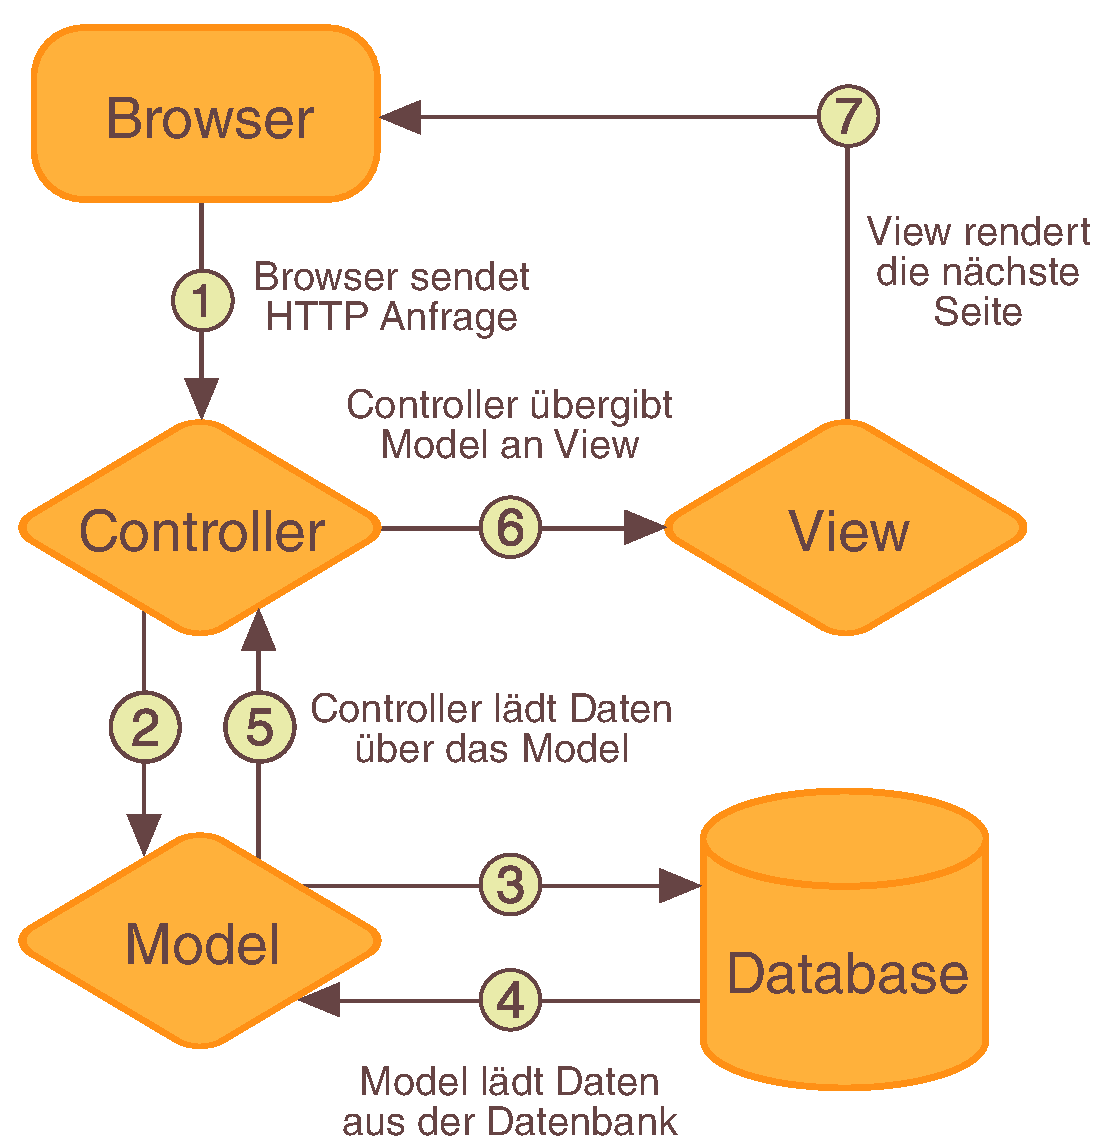
\includegraphics[width=300px]{bilder/mvc}
    \caption{MVC-Architektur in Ruby on Rails Applikationen}
  \end{center}
\end{figure}

\subsection{Representational State Transfer}
\label{rest}

Das Akronym \textit{REST} steht für \textit{Representational State
  Transfer} und stammt ursprünglich aus der Doktorarbeit
\textit{Architectural Styles and the Design of Network-based Software
  Architectures} \cite{Fielding2000}
\footnote{\url{http://www.ics.uci.edu/~fielding/pubs/dissertation/top.htm}}
von Roy T. Fielding. In dieser Arbeit werden verschiedene
Architekturstile für das Design netzwerkbasierter Hypermedia Systeme
vorgestellt und deren Verhalten bezüglich Effizienz, Skalierbarkeit
und einiger weiterer Kriterien untersucht. In Kapitel 5 wird
\textit{REST} als Architekturstil vorgestellt, der bewährte Konzepte
aus den zuvor anayliserten Architekturen aufgreift und Regeln und
Anforderungen für das Design moderner Web- Architekturen und
Anwendungen vorgibt. Fielding, der auch an der Spezifikation des
\textit{Hypertext Transfer Protocol (HTTP)}
\nomenclature{HTTP}{Hypertext Transfer Protocol} beteiligt war, führt
den großen Erfolg des \textit{World Wide Web (WWW)}
\nomenclature{WWW}{World Wide Web} unter anderem auf dessen
Architektur und die verwendeten Technologien zurück, die sich in den
von ihm vorgeschlagenen Regeln widerspiegeln.

\subsubsection{Resource-Oriented Architecture}

In \textit{RESTful Web Services} \cite{Richardson07} werden Fielding's
Vorschläge auf die Architektur moderner \textit{Web Services}
übertragen und \textit{Resource-Oriented Architecture (ROA)} als ein
konkreter Architekturstil vorgestellt, der sich an den Konzepten von
\textit{REST} orientiert. Im folgenden sollen die zugrunde liegenden
Konzepte und deren Anwendung anhand einiger Beispiele vorgestellt
werden.

\paragraph{Ressourcen}

Der Begriff \textit{Ressource} ist eine Abstraktion und wird in
\textit{ROA} verwendet um Dinge zu bezeichnen, die auf einem Computer
gespeichert, in einer Folge von Bits repräsentiert und auf irgendeine
Art und Weise identifiziert und referenziert werden können. Dokumente
auf einem Web Server, Zeilen einer Datenbanktabelle oder das Ergebnis
eines Algorithmus auf einer bestimmten Eingabe können als Ressource
modelliert werden. Einige konkrete Beispiele für eine Ressource sind:

\begin{itemize}
\item Die Version 3.0.12 eines Softwarepakets.
\item Die letzte stabile Version eines Softwarepakets.
\item Die Beschreibung der Surfbedingungen in \textit{Mundaka,
    Spanien}.
\item Die Wettervorhersage für \textit{Mundaka} am 26. Juli 2009 um 15:00h.
\end{itemize}

\paragraph{Identifizierung}
\label{paragraph:identifizierung}
Ressourcen müssen identifiziert werden können. Im Web werden hierfür
üblicherweise \textit{Uniform Resource Identifier (URI)}
\nomenclature{URI}{Uniform Resource Identifier} verwendet. Eine
Ressource muß mindestens einen \textit{URI} besitzen, die von
Anwendungen verwendet wird um Informationen über eine Ressource zu
bekommen oder diese zu verändern. Die eben als Beispiel erwähnten
Ressourcen könnten z.B. über die folgenden \textit{URI}s identifiziert
werden:

{\sf \small
  \begin{itemize}
  \item http://example.com/software/releases/3.0.12.tar.gz
  \item http://example.com/software/releases/latest.tar.gz
  \item http://example.com/spots/03-Mundaka/description.html
  \item http://example.com/spots/03-Mundaka/forecasts/2009-07-26/15h.html
  \end{itemize}
}

Wie an den ersten beiden Beispielen zu sehen ist, kann eine Ressource
zu einem bestimmten Zeitpunkt auch über mehrere \textit{URI}s
identifiziert werden: Zu einem bestimmten Zeitpunkt war Version 3.0.12
der Software auch die aktuellste Version. Der Aufbau oder die Struktur
von \textit{URI}s wird durch \textit{REST} nicht strikt vorgegeben.
Eine durch den Clienten vorhersehbare Struktur wird aber in
\textit{ROA} empfohlen, da dies zum einen gutes Design ausmacht und
zugleich dem Clienten die Möglichkeiten gibt flexibel auf den Web
Service zuzugreifen.

\paragraph{Adressierbarkeit}

Ein \textit{Web Service} ist addressierbar wenn die zur Verfügung
gestellten Informationen als Ressourcen publiziert werden und auf
diese durch \textit{URI}s zugegriffen werden kann. Die Anzahl der
\textit{URI}s, die von solch einem \textit{Web Service} angeboten
werden ist durch die Vielzahl der möglichen Eingaben meist unbegrenzt.
Vertreter solch eines \textit{Web Services} ist z.B. die Suche nach
dem Wort ''REST'' bei \textit{Google}, welche durch folgenden
\textit{URI} adressierbar ist:
\url{http://www.google.de/search?q=REST}.

Addressierbarkeit ist eine wichtige Eigenschaft
\textit{REST}-basierter Web Architekturen und bringt viel mehr
Anwendungsmöglichkeiten mit sich, als das ''bloße Publizieren'' von
Informationen. Beispiele hierfür sind:

\begin{itemize}
\item Die Informationen referenzierenden Adressen können z.B. in
  Büchern abgedruckt, als Lesezeichen gespeichert, per Mail
  weitergeleitet und als Eingabe für Programme dienen, welche den
  Inhalt weiterverarbeiten. Dadurch muss nicht der eigentliche Inhalt
  verbreitet oder kommuniziert werden werden sondern nur die Adresse
  unter der dieser Inhalt zu finden ist.
\item In \textit{HTTP Proxy Caches} wird die Adressierbarkeit von
  Ressourcen ausgenutzt um den Zugriff darauf zu beschleunigen. Bei
  einer ersten Anfrage wird die Ressource vom Proxy
  zwischengespeichert und weitere Anfragen an diese aus dem Cache
  bedient.
\item Durch \textit{URI}s adressierbare \textit{Web Services} bieten
  nicht nur den speziell entworfenen Programmen Zugang zu Ressourcen,
  sondern auch Menschen die mit Standardwerkzeugen wie z.B. einem
  \textit{Web Browser} oder einem \textit{RSS Reader} darauf zugreifen
  oder Agenten des \textit{Semantic Web}.
\end{itemize}

\paragraph{Zustandslosigkeit}

Unter Zustandslosigkeit bzw. \textit{Statelessness} versteht man in
Protokollen zur Client-Server Kommunikation, dass alle Anfragen des
Clienten an den Server komplett unabhängig voneinander sind. Anfragen
des Clienten müssen alle nötigen Informationen beinhalten, die vom
Server benötigt werden um diese zu bearbeiten. Auf Seiten des Servers
wird keinerlei Information über den Zustand von Anfragen
verwaltet. Dadurch wird dessen Implementierung vereinfacht, spart
Ressourcen beim Verarbeiten von Anfragen ein und bietet die
Möglichkeit \textit{Load Balancing} in Form von horizontaler
Skalierung zu betreiben. Zustandslosigkeit ist ebenfalls eine der von
Fielding geforderten Eigenschaften \textit{REST}-basierter
Architekturen.

\paragraph{Repräsentation}

Das abstrakte Konzept einer Ressource wird durch ihre Repräsentation
bzw. Darstellung konkretisiert. Fordert ein Client Informationen über
eine Ressource an, wird nicht die Ressource selbst, sondern eine
bestimmte Repräsentation dieser Ressource als Sequenz von Bytes
übertragen. Eine Ressource kann viele verschiedene Repräsentationen
haben, beispielsweise als \textit{HTML-},
\nomenclature{HTML}{Hypertext Markup Language} \textit{XML-} oder
\textit{JSON-}Dokument \nomenclature{JSON}{Javascript Object Notation}
kodiert. Die Darstellungen in unterschiedlichen Sprachen sind
ebenfalls mögliche Repräsentationen einer Ressource.

In \textit{ROA} wird empfohlen die Information welche Repräsentation
einer Ressource der Server ausliefern soll, in den \textit{URI} oder
in die Metadaten des verwendeten Übertragungsprotokolls
einzubetten. Mögliche Repräsentationen der Wettervorhersage für
\textit{Mundaka} am 26. Juli 2009 um 15:00h könnten z.B. als
''Dateiendung'' im \textit{URI} kodiert werden:

{\sf \small
  \begin{itemize}
  \item http://example.com/spots/03-Mundaka/forecasts/2009-07-26/15h.html
  \item http://example.com/spots/03-Mundaka/forecasts/2009-07-26/15h.xml
  \item http://example.com/spots/03-Mundaka/forecasts/2009-07-26/15h.json
  \end{itemize}
}

Durch Differenzierung von Repräsentationen einer Ressource kann ein
\textit{Web Service} Anwendungen mit verschiedenen Anforderungen
bedienen. \textit{Web Browsern} kann z.B. eine aufwendigere, auf
Interaktivität fokussierte Darstellung gesendet werden,
datenverarbeitenden Programmen eine Variante in \textit{XML} und
mobilen Endgeräten eine leicht-gewichtigere Version im \textit{JSON}
Format.

\paragraph{Einheitliche Schnittstelle}

Eine einheitliche Schnittstelle zwischen den Komponenten einer
\textit{REST}-basierten Architektur ist eine weitere Forderung
Fieldings, mit dem Ziel die Komplexität des zu entwerfenden Systems zu
reduzieren. Das Akronym \textit{CRUD} \nomenclature{CRUD}{Create,
  Read, Update, Delete} steht für die mindestens zu implementierenden
Operationen einer vollständigen \footnote{im Sinne der Theorie}
relationalen Datenbank: \textit{Create}, \textit{Read},
\textit{Update} und \textit{Delete}. Mit diesen Basis Operationen
können die Objekte einer Datenbank erstellt, gelesen, verändert und
gelöscht werden. Ausgehend von der Annahme, dass Ressourcen in einer
bestimmten Repräsentation auch in einer relationalen Datenbank
gespeichert werden können, bieten sich die \textit{CRUD}-Operationen
auch beim Design einer einheitlichen Schnittstelle für Ressourcen
an. In \cite{Richardson07}[S.97-105] wird das \textit{HTTP}-Protokoll
zur Implementierung der einheitlichen Schnittstelle
vorgeschlagen. Dabei werden die vier \textit{CRUD}-Operationen auf die
im \textit{HTTP}-Protokoll definierten \textit{GET}, \textup{POST},
\textit{PUT} und \textit{DELETE} Methoden abgebildet.

\begin{itemize}
\item Die Repräsentationen existierender Ressourcen werden mit der
  \textit{GET} Methode angefordert, beispielsweise die \textit{HTML}
  Repräsentation der Beschreibung zu den Surfbedingungen in
  \textit{Mundaka}.

  \texttt{GET http://example.com/spots/03-Mundaka.html}

\item Existierende Ressourcen werden mit der \textit{DELETE} Methode
  gelöscht. Im folgenden Beispiel wird der Surf Spot \textit{Mundaka}
  gelöscht.

  \texttt{DELETE http://example.com/spots/03-Mundaka}

\item Der Zustand existierender Ressourcen wird mit der \textit{PUT}
  Methode verändert. Im \textit{HTTP-Body} der Anfrage wird eine
  Repräsentation \footnote{In Web Applikationen üblicherweise in XML
    oder Form-Encoded} der Ressource mitgsesendet, die den veränderten
  Zustand widerspiegelt. Im folgenden Beispiel wird der Spot
  \textit{Mundaka} mit der im \textit{HTTP-Body} enthaltenen, hier
  aber nicht gezeigten, Repräsentation aktualisiert.

  \texttt{PUT http://example.com/spots/03-Mundaka}

\item Neue Ressourcen werden entweder mit der \textit{POST}- oder der
  \textit{PUT} Methode erstellt. Eine den Zustand der Ressource
  widerspigelnde Repräsentation wird hier ebenfalls im
  \textit{HTTP-Body} kodiert.

  Mit welcher Methode und \textit{URI} die Anfrage gesendet wird, ist
  abhängig davon ob der Client (\textit{PUT}) oder der Server
  (\textit{POST}) den \textit{URI} der neuen Ressource festlegt. Diese
  Unterscheidung ist auf die Einhaltung der im \textit{RFC-2616}
  \nomenclature{RFC}{Request for Comments} beschriebenen
  \textit{HTTP/1.1} Spezifikation zurückzuführen und wird in
  \cite{Richardson07}[S.99-102] ausführlicher erläutert. Die zwei
  folgenden Beispiele sollen beide Situationen verdeutlichen.

  \textbf{POST:} Der \textit{URI} für Spots wird in der hier
  entwickelten Web Applikation aus dem Datenbank Identifikator und dem
  Namen des Spots zusammengesetzt. Da der Datenbank Identifikator dem
  Benutzer beim Erstellen des neuen Spots nicht bekannt ist, muss hier
  die \textit{POST} Methode verwendet werden.

  \texttt{POST http://example.com/spots}

  \textbf{PUT:} Bei der Registrierung von Benutzern hingegen wird die
  \textit{PUT} Methode verwendet. Der \textit{URI} eines Benutzer wird
  in der Web Applikation nur aus dem von ihm gewählten Nicknamen
  konstruiert. Hier legt also der Client den \textit{URI} der neuen
  Ressource fest.

  \texttt{ PUT http://example.com/users/bob}

\end{itemize}

\section{Behaviour \& Test Driven Development}

\textit{Behaviour Driven Development} ist eine Erweiterung des
\textit{Test Driven Development}, einer Methode aus dem Bereich der
\textit{Agilen Softwareentwicklung}. Ziel der Agilen
Softwareentwicklung ist es den klassischen Softwareentwicklungsprozess
schlanker und flexibler zu gestalten und sich mehr auf die zu
erreichenden Ziele und Anforderungen zu
fokussieren. Paarprogrammierung, ständige Refaktorisierung des Codes
und testgetriebene Entwicklung sind einige der dabei verwendeten
Methoden \cite{wiki:agile}.

Behaviour Driven Development ist ein durch Dan North geprägter Begriff
und eine Erweiterung der Philosophie des Test Driven Developments
\cite{wiki:bdd}. Durch die Einführung eines gemeinsamen Vokabulars
soll die Zusammenarbeit zwischen Programmieren und nicht-technischen
Beteiligten an einem Softwareprojekt erhöht werden. Das gemeinsame
Vokabular wird benutzt um das Verhalten, bzw. die Anforderungen der
Software gemeinsam zu beschreiben und eine Spezifikation zu erstellen.

Diese Spezifikation wird in Form von automatischen Tests in einer
domänen\-spezifische Sprache vom Programmierer implementiert.

\subsection{Red, Green, Refactor}

Die Entwicklung der Software erfolgt, wie beim Test Driven
Development, durch ständige Wiederholung des \textit{Red, Green,
  Refactor} Zykluses. \textit{Red} und \textit{Green} stehen für
fehlschlagende bzw. erfolgreiche Testfälle, und \textit{Refactor} für
die Umstrukturierung, Verbesserung und Säuberung schon implementierten
Programmcodes. Die Entwicklung der Anwendung wird in kleinere Teile,
sogenannte \textit{Feature} aufgeteilt und diese nacheinander
abgearbeitet. Das Verhalten eines zu implementierenden Features wird
durch mehrere Testfälle beschrieben und somit spezifiziert. Dabei
werden die folgenden drei Schritte solange wiederholt bis das
gewünschte Feature ausreichend spezifiziert und implementiert ist. Die
Kunst ist hierbei, immer nur sehr kleine Schritte pro Zyklus zu
spezifizieren und zu implementieren.

\subsubsection{Red - Die Spezifikation des Verhaltens}

In der \textit{Red} Phase wird ein korrekter, aber fehlschlagender,
Test geschrieben, der ein bestimmtes Verhalten eines noch nicht
implementiertes Features spezifiziert. Dieser Test sollte nur einen
sehr geringen Teil des gesamten Features
verifizieren. Beispielsweise, dass eine Methode ein Array zurück gibt,
die Elemente eines Arrays Instanzen einer bestimmten Klasse sind oder
die Distanz zwischen zwei gegebenen geografischen Positionen korrekt
berechnet wird.

\subsubsection{Green - Die Implementierung des Verhaltens}

Ziel der \textit{Green} Phase ist es den soeben geschriebenen und
fehlschlagenden Test (und alle bisher erfolgreichen) durch eine
geeignete Implementierung zum Erfolg zu bringen. Hierbei ist zu
Erwähnen, dass auch eine vorübergehend nicht korrekte Implementierung
erlaubt ist, solange alle Tests erfolgreich sind. Beispielsweise kann
eine Methode vorübergehend immer einen leeren Array zurückgegeben,
wenn im Test nur auf die Rückgabe eines Arrays geprüft wird. Diese
inkorrekten Implementierungen sind gewollte Indizien für die als
nächstes zu spezifizierenden Testfälle. In einem der nächsten Zyklen
wird die inkorrekte Implementierung durch einen neuen fehlschlagenden
Test aufgedeckt und durch eine korrekte Implementierung ausgetauscht.

\subsubsection{Refactor - Besserer Programmcode durch
  Umstrukturierung}

Die \textit{Refactor} Phase dient dazu, bisher entwickelten
Programmcode durch Umstrukturierung aufzuräumen. Dazu zählt die
Eliminierung doppelten oder ähnlichen Codes, das Extrahieren von
Hilfsmethoden und weiterer Refactor-Techniken, die ausführlich in
\cite{Fowler1999} beschrieben werden. Insbesondere in Software
Projekten, die ohne automatische Tests entwickelt werden, ist diese
Phase hoch problematisch. Zuvor funktionierender und durch Refactoring
geänderter Programmcode muss nochmals manuell verifiziert
werden. Probleme treten oft auch an nicht offensichtlich mit den
Änderungen in Verbindung stehenden Teilen des Programms auf. Ein
deshalb notwendiger, manueller Systemtest kann dann oft zu aufwendig
sein, dass die Vorteile des Refactoring in den Hintergrund rücken und
oftmals darauf verzichtet wird.  \textit{''Never change a running
  system''. \footnote{Oft falsch verwendeter Pseudoanglizismus}}

\subsection{Vorteile Behaviour \& Test Driven Developments}

Diese Art der Softwareentwicklung wird heute oft immer noch aus den
verschiedensten Gründen abgelehnt. \textit{''Nicht notwendig, bei gut
  entwickeltem Code''}, \textit{''zu aufwendig''}, oder Barrieren,
seine gewohnte Arbeitsweise zu ändern, sind einige dieser Gründe. Der
Klassiker \textit{''man würde ja, aber habe keine Zeit Tests zu
  schreiben''} zeigt, dass die Vorteile des Test Driven Development
oft nicht erkannt werden. Dies liegt unter anderem wohl daran, dass es
einige Zeit in Anspruch nimmt seine gewohnte Arbeitsweise zu ändern,
und die Früchte erst nach einiger Zeit und Praxis deutlich zu sehen
sind. Einige der Vorteile sollen im folgenden deutlich gemacht werden.

\subsubsection{Steigerung der eigenen Produktivität}

Martin Fowler beschreibt in \cite{Fowler1999}[S.89], dass viele
Programmierer ihre Zeit nicht mit der Entwicklung des eigentlichen
Programmcodes verbringen. Ein Großteil der Zeit wird für Debugging und
das manuelle Testen des gerade zu entwickelten Codes
verwendet. Produziert wird hier nur der eigentliche Programmcode. Beim
Test Driven Development wird diese Zeit für die selben Ziele
verwendet, doch als Nebenprodukt entstehen automatische
Tests. Manuelles Testen und Debugging muss unter Umständen immer
wieder von neuem wiederholt werden, während automatische Tests
sicherstellen, dass bestimmte Dinge funktionieren und nicht nochmals
verifiziert werden müssen. Die Entwicklung von Tests bedeutet mehr
Code, was mit mehr Arbeit gleichzusetzen ist. Dieser Mehraufwand
scheint auf den ersten Blick keinen Sinn zu machen, bis man selbst
erfahren hat wie sehr dieses Vorgehen die eigene Produktivität
steigern kann.

\subsubsection{Besserer Programmcode}

Schreibt man Tests vor der eigentlichen Implementierung blickt man von
vornherein aus der Rolle eines Anwenders auf die zu entwickelnde
Schnittstelle. Die API des zu implementierenden Codes kann so während
der Entwicklung der Testfälle ''erforscht'' werden. Die Struktur des
Programmcodes wird zudem positiv beeinflusst, da vor der
Implementierung überlegt werden muss wie das Verhalten am besten
getestet werden kann. Implementierungen, die vor Testfällen entwickelt
wurden, müssen oft umstrukturiert werden damit diese überhaupt
getestet werden können. Zu lange Methoden sind hier das klassische
Beispiel. Sie lassen sich schlecht testen weil sie oft viel zu viel
auf einmal erledigen. Darüber hinaus sind sie meist auch noch schwer
zu verstehen. Durch Extraktion von Hilfsmethoden kann man diese
Methoden verkürzen und verbessert dadurch die Lesbarkeit des
Codes. Die extrahierten Methoden und die verkürzte Methode selbst
lassen sich nun in Isolation meist viel besser und einfacher testen
als zuvor. Zudem können die extrahierten Hilfsmethoden potentiell von
anderem Programmcode mitverwendet werden.

\subsubsection{Qualitätsmanagment und Teamwork}

Insbesondere bei Softwareprojekten in dynamischen Programmiersprachen,
die erst zur Laufzeit interpretiert werden und keine statische
Typprüfung besitzen ist es von großem Vorteil eine automatische
Testsuite zu haben. In diesen Sprachen gibt es keinen Compiler der
nach Änderungen überprüfen kann, dass zumindest syntaktisch noch alles
korrekt ist. Änderungen an einer Stelle im System haben oft
Konsequenzen an anderen nicht vorhersehbaren Stellen. Eine Testsuite,
welche die gesamte Codebasis abdeckt kann sicherstellen, dass
Änderungen funktionieren und eingeschlichene Fehler so früh wie
möglich aufgedeckt werden.

Auch bei Softwareprojekten, die von mehreren Personen gleichzeitig
entwickelt werden bietet eine Testsuite Schutz gegen das Einschleichen
von Fehlern und hilft bei der Weiterentwicklung fremden Codes. Wird
Programmcode vom nicht ursprünglichen Autor geändert oder erweitert
muss dieser zuerst verstanden, erweitert und danach verifiziert
werden. Testfällen dienen dabei nicht nur zur Verifizierung dieser
Änderungen, sondern auch als Dokumentation und Spezifikation, und
helfen somit das Problem besser und schneller zu verstehen.

\subsection{Unit Tests mit RSpec}

\textit{RSpec} \cite{rspec} ist ein Behaviour Driven Development
Framework für die Entwicklung von Softwareprojekten in der
Programmiersprache Ruby.  Es implementiert eine interne
bzw. eingebettete domänen\-spezifische Sprache (DSL) zur Spezifikation
von Anforderungen in Form von Unit Tests.  Spezifikationen können wie
bei den diversen xUnit Derivaten gruppiert, verifiziert und deren
Resultate angezeigt werden. Als Beispiel soll hier die Implementierung
einer Klasse dienen, welche die Distanz in Kilometern zwischen zwei
geografischen Positionen berechnet. Vor der eigentlichen
Implementierung wird das Verhalten der Klasse anhand von Beispielen in
der RSpec DSL wie folgt spezifiziert:

\begin{lstlisting}
describe Haversine do
  it "should calculate a distance of 0 km between the same location"
  it "should calculate a distance of 878.01 km between Berlin and Paris"
end
\end{lstlisting}

Diese Spezifikation der Haversine Klasse ist Teil des oben erwähnten
gemeinsamen Vokabulars und zugleich gültiger und ausführbarer Ruby
Code. Die Entwicklung einer einfachen, verständlichen und
aussagekräftigen DSL hatte zum Ziel, dass Spezifikationen wie diese
von oder mit nicht-technischen Personen erstellt werden können. Die
eigentliche Verifizierung und Implementierung des Verhaltens soll dann
vom Programmierer erstellt werden. Bevor die Haversine Formel durch
eine Klasse implementiert wird, erweitert der Programmierer die
Spezifikation durch Code, der das Verhalten der Klasse verifiziert. Da
die Spezifikation in der Programmiersprache Ruby geschrieben ist, kann
diese vom Programmierer einfach und flexibel erweitert werden. Auch
hier kommen Konstrukte der RSpec DSL zum Einsatz, welche die
Lesbarkeit vereinfachen und die Spezifikation verständlicher machen
sollen.

\begin{lstlisting}
describe Haversine do

  before(:each) do
    @berlin = Location.make(:berlin)
    @paris = Location.make(:paris)
  end

  it "should calculate a distance of 0 km between the same location" do
    Haversine.distance(@berlin, @berlin).should == 0.km
  end

  it "should calculate a distance of 878.01 km between Berlin and Paris" do
    Haversine.distance(@berlin, @paris).should == 878.01.km
  end

end
\end{lstlisting}

Das Ausführen dieser Spezifikation schlägt auf Grund der noch
fehlenden Implementierung fehl. Durch die Wiederholung des Red, Green,
Refactor Zykluses wird nun das Verhalten der Klasse implementiert. Der
erste Testfall kann durch die folgende, noch inkorrekte
Implementierung zum Erfolg gebracht werden:

\begin{lstlisting}
class Haversine

  def self.distance(from, to, options = { })
    return 0 # A first, naive implementation.
  end

end
\end{lstlisting}

Im nächsten Iterationszyklus muß nun die eigentliche Haversine Formel
\cite{wiki:haversine} implementiert werden um auch den zweiten
Testfall zum Erfolg zu bringen. Durch das Aufteilen der zu
bewältigenden Aufgaben in kleine Iterationszyklen wird das
spezifizierte Verhalten so Schritt für Schritt implementiert. Die
nächste zu bearbeitende Teilaufgabe wird durch einen neuen Testfall
beschrieben und das bisher erwartete Verhalten durch die bestehenden
verifiziert.

Das im Umfeld von RSpec entwickelte \textit{Spec::Rails} Plugin bietet
die nötige Infrastruktur für Ruby on Rails Projekte. An die
MVC-Architektur von Rails angelehnt werden verschiedene Umgebungen und
Hilfsmethoden bereit gestellt um Model, View, Controller und Helper zu
spezifizieren. Während der Entwicklung des Prototypen der Web
Applikation wurden insgesamt 4274 Testfälle spezifiziert, die 92.6\%
(C0 Code Coverage) des gesamten Codes abdecken und das korrekte
Verhalten der Web Applikation verifizieren.

Das Durchlaufen der gesamten Testsuite benötigt momentan ca. 15
Minuten, was zu einem Durchschnitt von 4,8 Sekunden pro Test
führt. Diese hohe Laufzeit lässt sich auf die vielen Datenbankzugriffe
zurückführen, die vor den meisten Testfällen einen bestimmten
Datenbestand herstellen und danach wieder zurücksetzen müssen. Durch
den Einsatz von \textit{Mocks} und \textit{Stubs} können diese
Datenbankzugriffe reduziert werden. Diese Techniken sollten jedoch
vorsichtig eingesetzt werden. Eine übermäßige Anwendung resultiert
meist in einer zu engen Kopplung zwischen Test und
Implementierung. Diese Kopplung macht sich dann meist beim Refactoring
bemerkbar, wenn Tests ebenfalls geändert werden müssen weil aus
Performanzgründen Annahmen über die Implementierung getroffen
wurden. Hier muss man einen Mittelweg zwischen der Wartbarkeit der
Testsuite und deren Laufzeit finden.

In der Praxis hat sich herausgestellt, dass der Durchschnittswert von
4,8 Sekunden pro Test von geringer Bedeutung ist. Bei der
Implementierung eines Features lässt man meist nur die gerade
aktuellen Testfälle laufen und deren Laufzeit ist im einzelnen meist
besser als der erwähnte Durchschnittswert. Mindestens vor jedem
Deployment sollte dann die gesamte Testsuite ausgeführt werden um
sicherzustellen, dass das System auch in der Gesamtheit korrekt
funktioniert.

\subsection{Integrationstests mit Cucumber}

\textit{Cucumber} \cite{cucumber} ist ein weiteres Framework für
Behaviour Driven Development in Ruby. Es bietet die Möglichkeit das
Verhalten von Anwendungen in einer \textit{natürlichen Sprache}, wie
z.B. Englisch oder Deutsch, zu beschreiben. Auch hier war das Ziel,
das nicht-technische Personen das Verhalten einer Anwendung durch ein
gemeinsam verwendetes Vokabular beschreiben und spezifizieren können.
Die Spezifikationen wird dann von einem Entwickler erweitert um daraus
automatische Tests zu erstellen. In Ruby on Rails Projekten wird
Cucumber üblicherweise benutzt um durch Integrationstests
sicherzustellen, dass das Zusammenspiel zwischen Browser und
Controllern funktioniert.

Ein Feature wird in Cucumber's externer DSL \textit{Gherkin}
\footnote{\url{http://wiki.github.com/aslakhellesoy/cucumber/gherkin}}
beschrieben, einer sogenannten \textit{Business Readable, Domain
  Specific Language}.
\footnote{\url{http://martinfowler.com/bliki/BusinessReadableDSL.html}}
Die Beschreibung kann in einer der über 30 unterstützen natürlichen
Sprachen verfasst werden, wobei nur eine durch Gherkin definierte
Struktur eingehalten werden muss. Als Beispiel für solch eine
Spezifikation soll hier die Authentifizierung eines Benutzers durch
die Web Applikation dienen.

\begin{lstlisting}[caption=Spezifikation eines Features mit Cucumber]
Feature: Authentication
  To ensure the safety of the application
  A user of the system
  Must authenticate before using the application

  Scenario: Login as an activated user with wrong credentials
    Given I am an activated user
     When I log in with invalid credentials
     Then I should see "Sorry, invalid nick/password
          combination given."
      And I should not be logged in
\end{lstlisting}

Die Struktur der Beschreibung ist durch die Reihenfolge einiger
Schlüssel\-wörter vorgegeben. Mit dem Schlüsselwort \textit{Feature}
wird die Spezifikation eines Features eingeleitet, gefolgt von einer
kurzen Beschreibung zu Dokumentationszwecken. Ein Abschnitt, der mit
dem Schlüsselwort \textit{Scenario} definiert wird, beschreibt das
Verhalten der Anwendung in einer bestimmten Situation. Mit dem
Schlüsselwort \textit{Given} beschreibt man welche Vorbedingungen in
der gegebenen Situation herrschen müssen. \textit{When} beschreibt
auszuführende Aktionen, wie z.B. das Ausfüllen eines Formulars oder
das Klicken eines Links. Das Schlüsselwort \textit{Then} beschreibt
denn Zustand nach dem ausführen der Aktionen. Mit \textit{And} wird
eine weitere Zeile des selben Typs der vorigen Zeile definiert, und
dient zur Verknüpfung und der besseren Lesbarkeit.

Cucumber verarbeitet solch eine Spezifikation zeilenweise und führt
für bestimmte Zeilen Code aus der die beschriebenen Vorbedingungen
herstellt, Aktionen ausführt und Erwartungen verifiziert. Für jede
Zeile, die mit einem der Schlüsselwörter \textit{Given},
\textit{When}, \textit{Then} oder \textit{And} anfängt, muss ein auf
sie passender regulärer Ausdruck definiert werden, der mit einem
Codeblock assoziiert wird.

Der folgende Programmcode definiert einen regulären Ausdruck der auf
die erste \textit{Given} Zeile passt. Der mit ihm assoziierte Codeblock
erstellt einen neuen und aktivierten Benutzer, speichert ihn in der
Datenbank und weist ihn einer Variablen zu, auf die in anderen
Codeblöcken zugegriffen werden kann.

\begin{lstlisting}
Given /^I am an activated user$/ do
  @current_user = User.make(:activated)
end
\end{lstlisting}

Cucumber stellt eine Bibliothek einiger dieser häufige verwendeten
Konstrukte als Makros zu Verfügung. Diese können in eigenen
Codeblöcken benutzt werden. Der folgende Code verwendet einige dieser
vordefinierten Konstrukte. Der Code der dabei ausgeführt wird
simuliert das Besuchen der \textit{Login} Seite, das Ausfüllen zweier
Textfelder mit dem Benutzernamen und einem falschen Passwort, sowie
das Klicken des \textit{Login} Buttons mit einem Browser.

\begin{lstlisting}
When /^I log in with invalid credentials$/ do
  Given "I am on the login page"
  When  "I fill in \"login\" with \"#{@current_user.nick}\""
  When  "I fill in \"password\" with \"invalid-password\""
  When  "I press \"Login\""
end
\end{lstlisting}

Die Zeile \textit{Then I should see ''Sorry, invalid nick/password
  combination given.''} verwendet ebenfalls ein von Cucumber
definiertes Makro, dass überprüft ob der in Hochkomma gesetzte Text in
der vom Server empfangenen HTML Seite zu finden ist.

Die letzte Zeile ist ein selbst definiertes Makro, das wiederum
Methoden des RSpec Frameworks verwendet um zu überprüfen dass der
Benutzer nicht angemeldet ist.

\begin{lstlisting}
Then /^I should not be logged in$/ do
  controller.send(:current_user).should be_nil
end
\end{lstlisting}

Cucumber bietet die Möglichkeit eigene Makros interaktiv zu
entwickeln. Für Zeilen die keinem regulären Ausdruck zugeordnet werden
können, generiert Cucumber auf sie passende Codeblöcke, die sehr
einfach angepasst und weiterentwickelt werden können. Durch die
Verwendung der eigenen und der vielen vordefinierten Makros lässt sich
so ein auf die eigene Domäne zugeschnittenes Vokabular definieren, mit
dem das korrekte Verhalten einer Anwendung auf einem hohem
Abstraktionsniveau verifiziert werden kann.

Da Cucumber relativ neu ist wurden im hier entwickelten Prototypen
bisher nur 17 solcher Szenarien spezifiziert, die vor allem die
korrekte Interaktion mit externen Diensten
verifizieren. Beispielsweise werden von Benutzern publizierte Videos
und Bilder von der Web Applikation auf \textit{Amazon's
  S3}\footnote{Amazon Simple Storage Service
  \url{http://aws.amazon.com/s3}} gespeichert. Die Verwendung dieses
Web Services wurde aus Performanzgründen in den RSpec Unit Tests durch
Mock Objekte ersetzt. Integrationstests mit Cucumber bieten hier eine
gute Möglichkeit das Zusammenspiel von Browser und Controllern in
einer realitätsnahen Umgebung zu verifizieren.

\section{Caching Verfahren in Ruby on Rails}

%%% Local Variables:
%%% mode: latex
%%% TeX-master: "../community-plattform"
%%% End:
